\section{Experimental Evaluation}
\label{sec:experiments}

We evaluate our certificate-based verification framework on two benchmark systems to demonstrate: (1) the effectiveness of transition safety and persistence certificates for LTL verification, (2) computational efficiency compared to prior closure certificate methods~\cite{murali2024closure}, and (3) the practical applicability of SMT-based synthesis. All experiments run on Ubuntu 22.04.3 LTS (Intel i7-9750H, 8 GB RAM). We use Z3~\cite{de2008z3} for linear arithmetic and dReal~\cite{gao2013dreal} ($\delta = 0.0001$) for nonlinear verification. Table~\ref{tab:results} compares synthesis times. Our certificates achieve \textbf{141$\times$ to 909$\times$ speedup} over closure certificates~\cite{murali2024closure}, confirming the efficiency gains from reduced search space complexity.
\begin{table}[h]
\centering
\caption{Synthesis time comparison (seconds).}
\label{tab:results}
\begin{tabular}{lccc}
\hline
\textbf{Benchmark} & \textbf{Our Method} & \textbf{Closure~\cite{murali2024closure}} & \textbf{Speedup} \\
\hline
Kuramoto 1D & 4.25 & 600 & 141$\times$ \\
Kuramoto 2D & 7.27 & 6600 & 909$\times$ \\
Two-Room & 8.77 & 5400 & 616$\times$ \\
\hline
\end{tabular}
\end{table}

\subsection{Kuramoto Oscillator: Safety Verification}

The Kuramoto model describes coupled oscillators in neuroscience and power systems~\cite{guo2021overviews}. We verify safety specifications $\mathbf{G}\neg a$ (always avoid unsafe states) for one-dimensional and two-dimensional scenarios.

\subsubsection{One-Dimensional System}

The system $\mathfrak{S} = (\mathcal{X}, \mathcal{X}_0, f)$ has state space $\mathcal{X} = [0, 2\pi]$, initial states $\mathcal{X}_0 = [\frac{4\pi}{9}, \frac{5\pi}{9}]$, unsafe states $\mathcal{X}_u = [\frac{7\pi}{9}, \frac{8\pi}{9}]$, and dynamics:
\begin{align}
f(x) = x + t_s\Omega + t_s K \sin(-x) - 0.532 x^2 + 1.69,
\end{align}
where $t_s = 0.1$ (sampling time), $\Omega = 0.01$ (natural frequency), $K = 0.0006$ (coupling strength).

\begin{figure}[t]
  \centering
  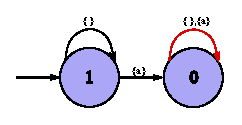
\includegraphics[width=0.3\textwidth]{pic/tbnba1.eps}
  \caption{NBA representing $\mathbf{F} a$ (negation of safety specification). Accepting transitions (red) form a self-loop at $q_0$.}
  \label{pic-tbnba1}
\end{figure}

With $AP = \{a\}$ and labeling $\mathfrak{L}(x) = \{a\}$ iff $x \in \mathcal{X}_u$, safety is expressed as $\mathbf{G}\neg a$. The negation $\mathbf{F} a$ is represented by the NBA in Figure~\ref{pic-tbnba1} with accepting transitions $(q_0, \{\}, q_0)$ and $(q_0, \{a\}, q_0)$ starting from $q_0 \in Acc^{start}$. We synthesize a transition safety certificate $B_0(x, q)$ using CEGIS with polynomial template:
\begin{align}
B_{0}(x, q; \mathbf{c}) = \sum_{i=0}^{4} c_i x^i + \sum_{j=1}^{3} c_{4+j} q^j + c_8 xq.
\end{align}
Sampling 629 states from $\mathcal{X}$ and 35 from $\mathcal{X}_0$, Z3 generates candidates and dReal verifies counterexamples. The synthesized certificate is:
\begin{align}
B_0(x, q) = -1 + 2q^2 - \frac{7}{16}xq.
\end{align}
CEGIS converges in \textbf{4.25 seconds}, proving safety. In contrast, closure certificate synthesis~\cite{murali2024closure} requires \textbf{10 minutes}—a \textbf{141$\times$ speedup}.

\subsubsection{Two-Dimensional System}

The system extends to $\mathcal{X} = [0, \frac{8\pi}{9}]^2$, $\mathcal{X}_0 = [0, \frac{\pi}{9}]^2$, $\mathcal{X}_u = ([0, \frac{8\pi}{9}] \times [\frac{5\pi}{6}, \frac{8\pi}{9}]) \cup ([\frac{5\pi}{6}, \frac{8\pi}{9}] \times [0, \frac{8\pi}{9}])$, with dynamics:
\begin{align}
f(x_1, x_2) =
\begin{bmatrix} x_1 \\ x_2 \end{bmatrix}
+ t_s
\begin{bmatrix} \Omega + 1.69 \\ \Omega + 1.69 \end{bmatrix}
+ K t_s
\begin{bmatrix} \sin(x_2 - x_1) \\ \sin(x_1 - x_2) \end{bmatrix}
- 0.532 t_s
\begin{bmatrix} x_1^2 \\ x_2^2 \end{bmatrix}.
\end{align}
The labeling marks $\mathfrak{L}(x_1, x_2) = \{a\}$ when $x_1 \in [\frac{5\pi}{6}, \frac{8\pi}{9}]$ or $x_2 \in [\frac{5\pi}{6}, \frac{8\pi}{9}]$, using the same NBA from Figure~\ref{pic-tbnba1}. CEGIS with template $B_{0}(x_1, x_2, q; \mathbf{c}) = c_0 + c_1 x_1 + c_2 x_2^2 + c_3 x_1 x_2 + c_4 x_1^3 + c_5 q + c_6 q^2 + c_7 q x_1^2 + c_8 x_2 q$ yields:
\begin{align}
B_0(x_1, x_2, q) = -1 + \frac{1}{8}x_1 x_2 + \frac{3}{2}q^2 - \frac{3}{32}q x_1^2 - \frac{153}{512}x_2 q.
\end{align}
CEGIS completes in \textbf{7.27 seconds}. The closure method requires \textbf{110 minutes}~\cite{murali2024closure}—a \textbf{909$\times$ speedup}.

\subsection{Two-Room Temperature: Persistence Verification}

We verify an interconnected temperature control system~\cite{anand2024compositional} where rooms must visit a comfort zone only finitely often from initial states. State space $\mathcal{X} = [20, 34]^2$ represents room temperatures, $\mathcal{X}_0 = [21, 24]^2$ are initial states, and:
\begin{align}
f(x_1, x_2) = A
\begin{bmatrix} x_1 \\ x_2 \end{bmatrix}
+ \mu T_h
\begin{bmatrix} u(x_1) \\ u(x_2) \end{bmatrix}
+ \theta
\begin{bmatrix} T_e \\ T_e \end{bmatrix},
\end{align}
where
\begin{align}
A = \begin{bmatrix} 1 - 2\alpha - \theta - \mu u(x_1) & \alpha \\ \alpha & 1 - 2\alpha - \theta - \mu u(x_2) \end{bmatrix},
\end{align}
with parameters $\alpha = 0.004$, $\theta = 0.01$, $\mu = 0.15$, $u(x_i) = 0.59 - 0.011 x_i$, $T_h = 40$, $T_e = 0$.

\begin{figure}[t]
  \centering
  
\includegraphics[width=0.3\textwidth]{pic/tbnba2.eps}
  \caption{NBA for $a \land \mathbf{GF} b$ (negation of $a \Rightarrow \mathbf{FG}\neg b$). Accepting transitions (red) are $(q_1, \{b\}, q_1)$ and $(q_1, \{a,b\}, q_1)$.}
  \label{pic-tbnba2}
\end{figure}

With $AP = \{a, b\}$, label $\mathfrak{L}(x_1, x_2) = \{a\}$ for $(x_1, x_2) \in \mathcal{X}_0$, $\mathfrak{L}(x_1, x_2) \ni b$ for $(x_1, x_2) \in [20, 26]^2$. The specification $a \Rightarrow \mathbf{FG}\neg b$ (from initial states, eventually stay outside comfort zone forever) has negation $a \land \mathbf{GF} b$ represented by the NBA in Figure~\ref{pic-tbnba2} with accepting transitions from $q_1$. First, we attempt transition safety synthesis to prove $q_1$ is unreachable. This \textbf{fails} after 16.24 seconds, indicating $q_1$ may be reachable. We then synthesize transition persistence certificates to prove accepting transitions occur finitely often.

Using SMT-based CEGIS with template $B_{1,1}(x_1, x_2; \mathbf{c}) = c_0 + \sum_{i=1,2} (c_i I_{\mathcal{X}_0} + c_{i+2} I_{[20,26]^2}) x_i + c_7 \max(x_1, x_2) + c_8 x_1^2 + c_9 x_2^2$, where $I_S$ is the indicator for set $S$, we obtain:
\begin{align}
B_{1,1}(x_1, x_2) = 27 I_{[20,26]^2}(x_1, x_2) - x_1 I_{[20,26]^2}(x_1, x_2), \quad \epsilon = 0.25.
\end{align}
Synthesis time: \textbf{8.77 seconds}. The closure method requires \textbf{90 minutes}~\cite{murali2024closure}—a \textbf{616$\times$ speedup}.

